%!TEX TS-program = Arara
% arara: pdflatex: {shell: yes}
\documentclass[12pt,ngerman]{beamer}

\usepackage[utf8]{inputenc}
\usepackage[T1]{fontenc}
\usepackage{booktabs}
\usepackage{babel}
\usepackage{graphicx}
\usepackage{csquotes}
\usepackage{paralist}
\usepackage{xcolor}
\usepackage{tikz}
\usetikzlibrary{calc}
\usepackage{listings}
\usepackage{pgfpages}
%\pgfpagesuselayout{2 on 1}

\lstset{%
    basicstyle=\ttfamily\scriptsize,%
    language={[LaTeX]TeX},%
    keywordstyle=\bfseries\color{red}, %
    morekeywords={forloop, begin, foreach,node,draw,pgfpageslogicalpageoptions,%
    pgfpagesphysicalpageoptions,pgfpageoptionborder,pgfphysicalwidth,%
    pgfusepath,pgfphysicalheight,pgfpoint,pgfpageoptionheight,%
    pgfpageoptionwidth,pgfpageoptionfirstshipout}%
}


\author{Uwe Ziegenhagen}
\title{Pocketmods mit \LaTeX\ und Python}
\subtitle{https://github.com/UweZiegenhagen/TalksAndArticles/2021-Dante-Herbst}

\begin{document}

\begin{frame}

\maketitle

\end{frame}

\begin{frame}
\frametitle{Über mich}

\begin{itemize}
\item Geboren im \enquote{Speckgürtel} Berlins
\item Seit 2008 in Köln
\item Business Analyst bei verschiedenen Finanzdienstleistern
\item Seit 2020 bei der Toyota Kreditbank im Bereich \textit{Business Intelligence \& Treasury}
\item \TeX nisches Interesse: Satzautomatisierung (mit Python)
\end{itemize}
\end{frame}

\begin{frame}
\frametitle{Pocketmod}

\includegraphics[width=0.975\textwidth]{pmod.jpg};

\end{frame}



\begin{frame}
\frametitle{Über Pocketmods}

\begin{itemize}
\item Pocketmod = cleveres Faltsystem
\item Macht aus einer DIN A4 oder DIN A3 Seite \\  Kalender bzw. Notizbuch
\item Online-Generator unter pocketmod.com
\item Falt-Tutorial unter https://www.youtube.com/watch?v=FHD-01Sc9dM
\item Mein erster Artikel zum Thema in DTK 3/2010
\end{itemize}
\end{frame}


\begin{frame}
\frametitle{Faltschema}

\begin{tikzpicture}
\node (image) at (0,0) {
\includegraphics[width=0.975\textwidth]{PocketMod_Pages.pdf}};
%\draw[step=1.0,green,thin] (-5,-4) grid (5,4);
\draw[red,thick] (-2.65,0) -- (2.65,0);

\end{tikzpicture}
\end{frame}

\begin{frame}
\frametitle{pgfpages: Physische und Logische Seiten}

\begin{itemize}
\item \texttt{pgfpages} ist Teil von TikZ
\item Greift in den Ausgabemechanismus ein
\item \enquote{Schubst} Seiten beliebig umher
\item Erlaubt z.B. \texttt{\textbackslash pgfpagesuselayout\{2 on 1\}} \\ $\Rightarrow$ 2 Seite auf 1 Seite darstellen
\end{itemize}
\end{frame}

\begin{frame}[containsverbatim]
\frametitle{Beispiel für Seite Nr. 1}

\begin{lstlisting}
\pgfpagesphysicalpageoptions{%
logical pages=8,%
physical height=\pgfpageoptionheight,%
physical width=\pgfpageoptionwidth,%
current logical shipout=\pgfpageoptionfirstshipout%
}
 
\pgfpageslogicalpageoptions{1}{%
border shrink=\pgfpageoptionborder,%
resized width=.25\pgfphysicalwidth,%
border code=\pgfusepath{stroke},%
resized height=0.5\pgfphysicalheight,%
center=\pgfpoint{.875\pgfphysicalwidth}{.75\pgfphysicalheight}%
}%
\end{lstlisting}

\includegraphics[width=0.33\textwidth]{PocketMod_Pages.pdf}

\end{frame}


\begin{frame}[containsverbatim]
\frametitle{Pocketmods mit TikZ -- TODO Liste}

\begin{lstlisting}[basicstyle=\ttfamily\footnotesize]
\begin{tikzpicture}
\draw[very thick](0,\i*2)-- ++(0,1.5)-- ++(1.5,0)
                            -- ++(0,-1.5)--cycle; 
\draw[very thick](2.5,\i*2)-- (22,\i*2);
\draw[very thick](23,\i*2)-- ++(0,1.5)-- ++(1.5,0) 
                             -- ++(0,-1.5)--cycle; 
\end{tikzpicture}
\end{lstlisting}

\begin{center}

\begin{tikzpicture}[scale=0.45]
\draw[very thick](0,0)-- ++(0,1.5)-- ++(1.5,0) -- ++(0,-1.5)--cycle; 
\draw[very thick](2.5,0)-- (22,0);
\draw[very thick](23,0)-- ++(0,1.5)-- ++(1.5,0) -- ++(0,-1.5)--cycle; 
\end{tikzpicture}
\end{center}

\end{frame}

\begin{frame}[containsverbatim]
\frametitle{Pocketmods mit TikZ -- 1. Schleife}

Eine Schleife, um eine Seite zu erzeugen.

\begin{lstlisting}[basicstyle=\ttfamily\footnotesize]
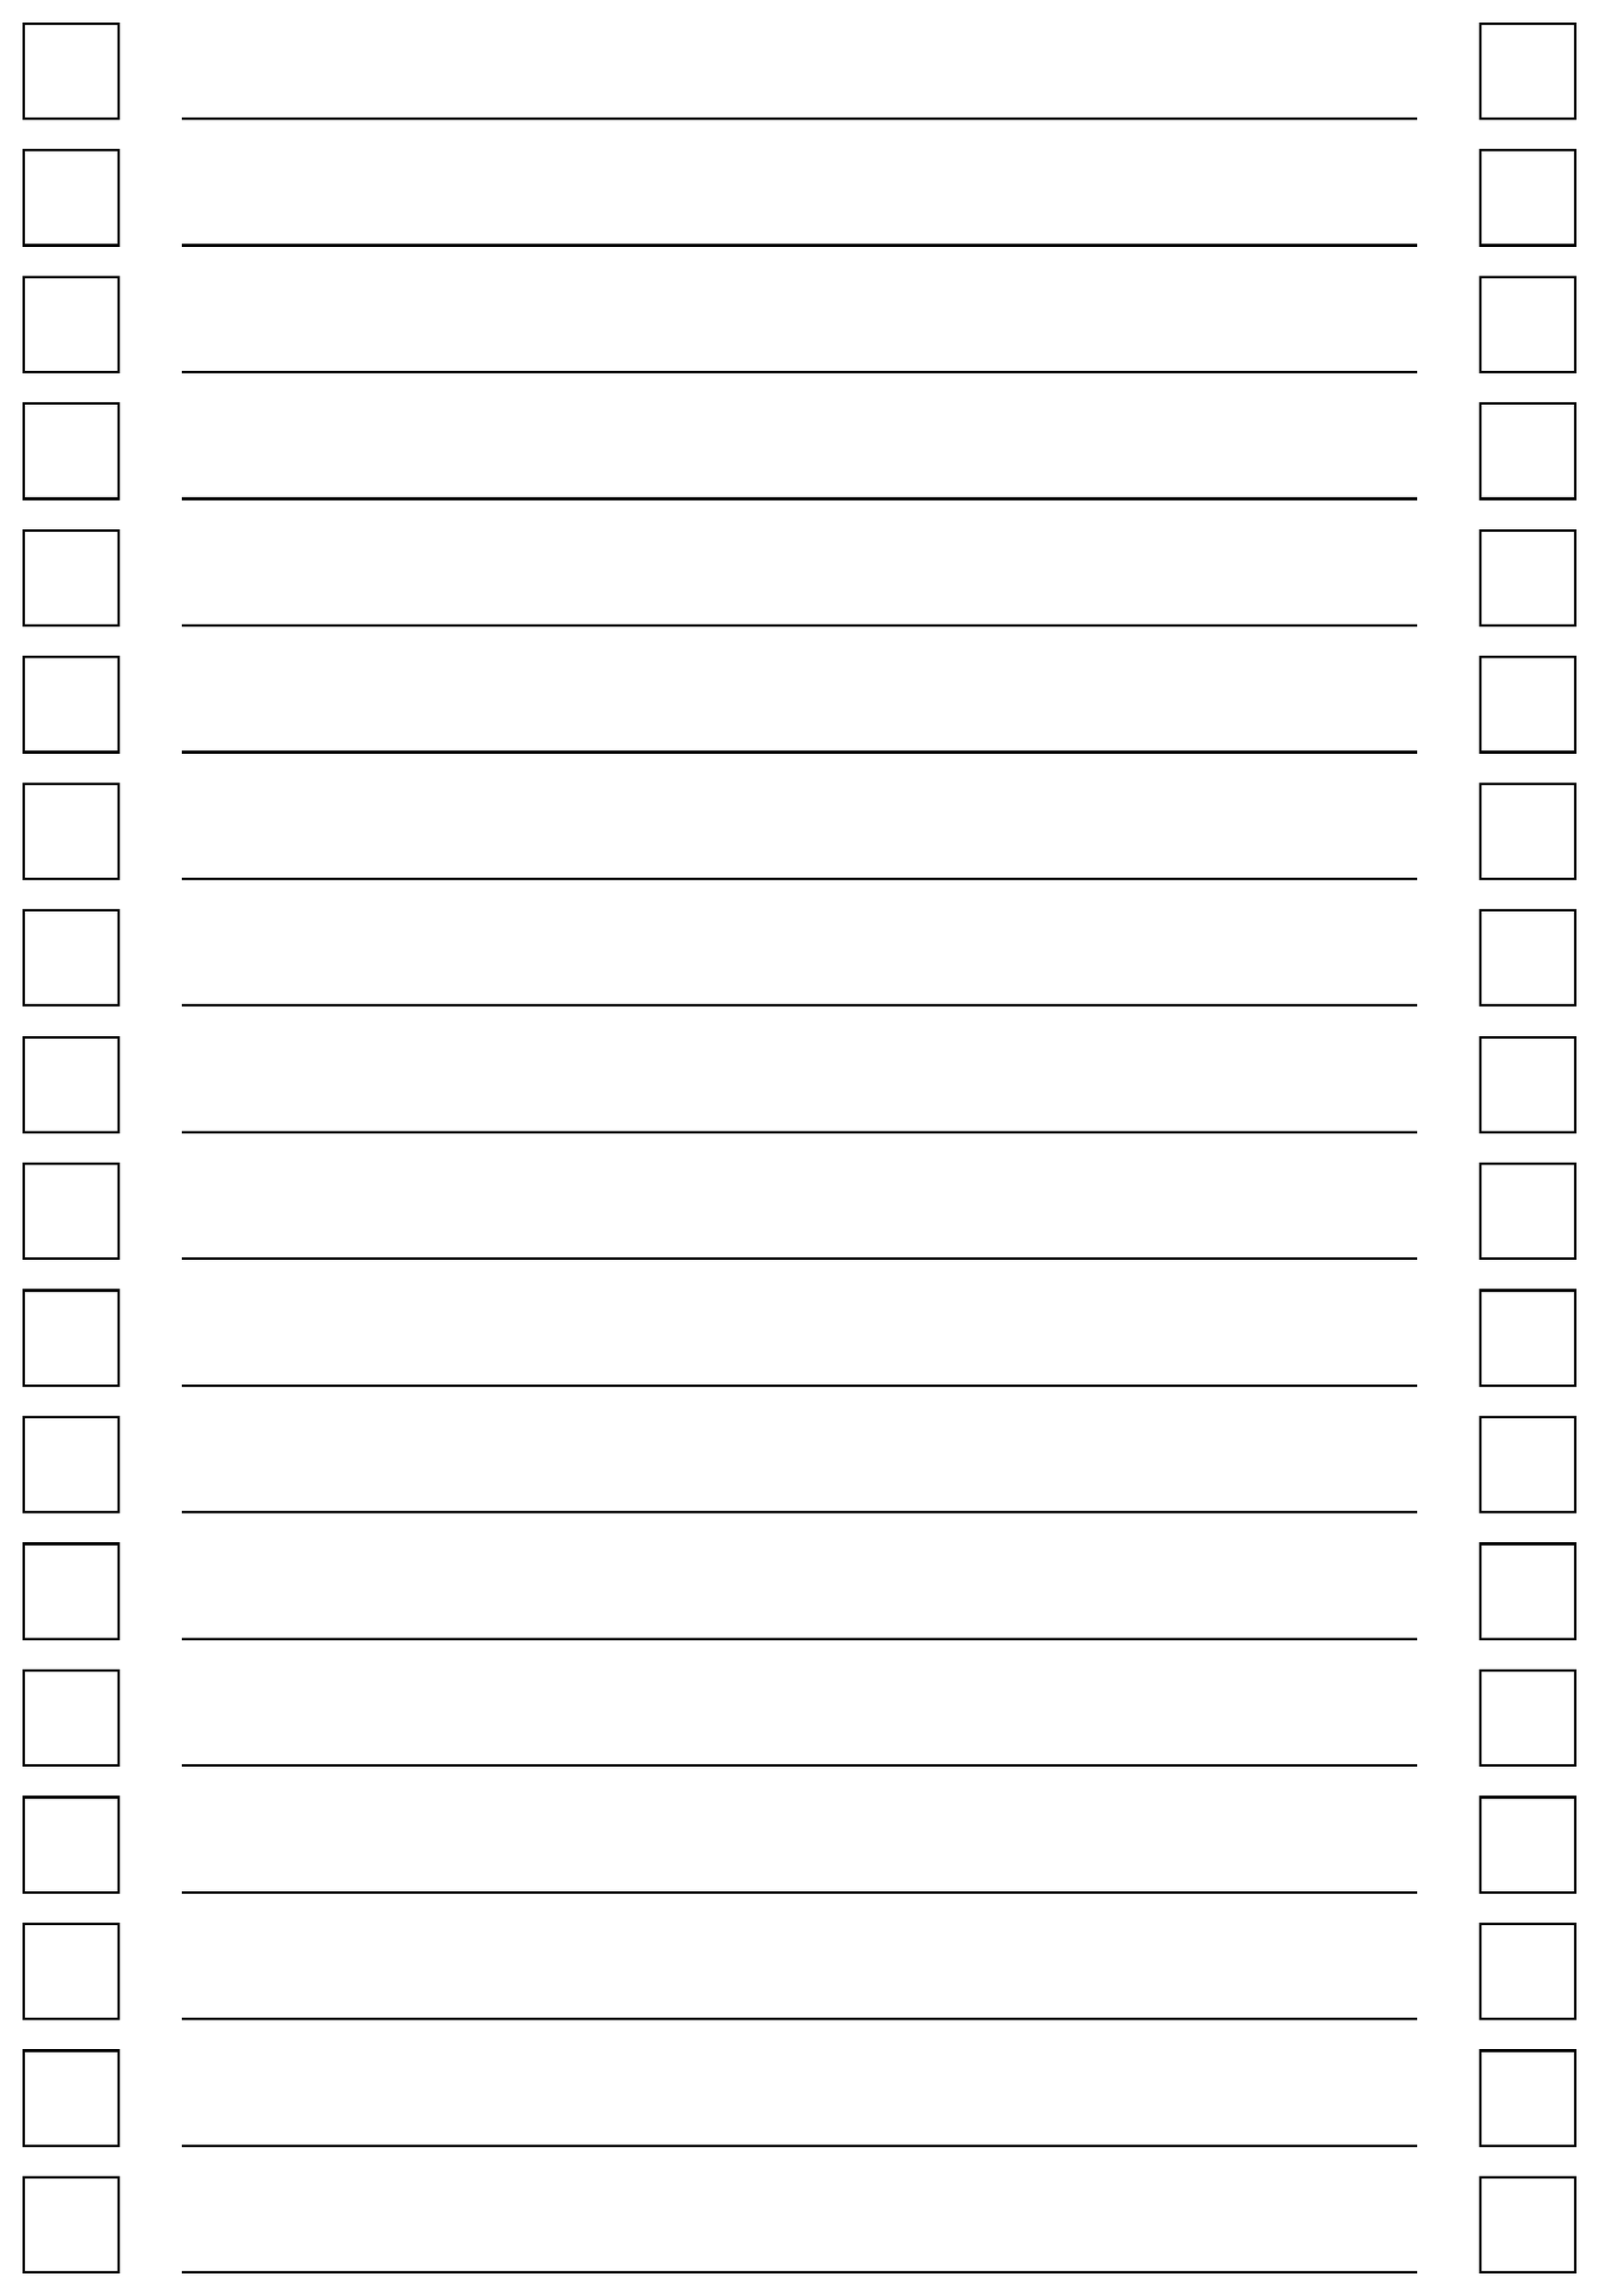
\begin{tikzpicture}
\foreach \i in {0,...,-17}{%
\draw[very thick](0,\i*2)-- ++(0,1.5)-- ++(1.5,0)
                            -- ++(0,-1.5)--cycle; 
\draw[very thick](2.5,\i*2)-- (22,\i*2);
\draw[very thick](23,\i*2)-- ++(0,1.5)-- ++(1.5,0) 
                             -- ++(0,-1.5)--cycle; 
}
\end{tikzpicture}
\end{lstlisting}
\end{frame}


\begin{frame}[containsverbatim]
\frametitle{Ergebnis der ersten Schleife}

\begin{center}
\fbox{\includegraphics[width=0.5\textwidth]{TODO_Liste.pdf}}
\end{center}

\end{frame}



\begin{frame}[containsverbatim]
\frametitle{Pocketmods mit TikZ -- 2. Schleife}

Zweite Schleife für die Erstellung der acht Seiten.
\begin{lstlisting}[basicstyle=\ttfamily\footnotesize]
\forloop{ct}{1}{\value{ct} < 9}{%
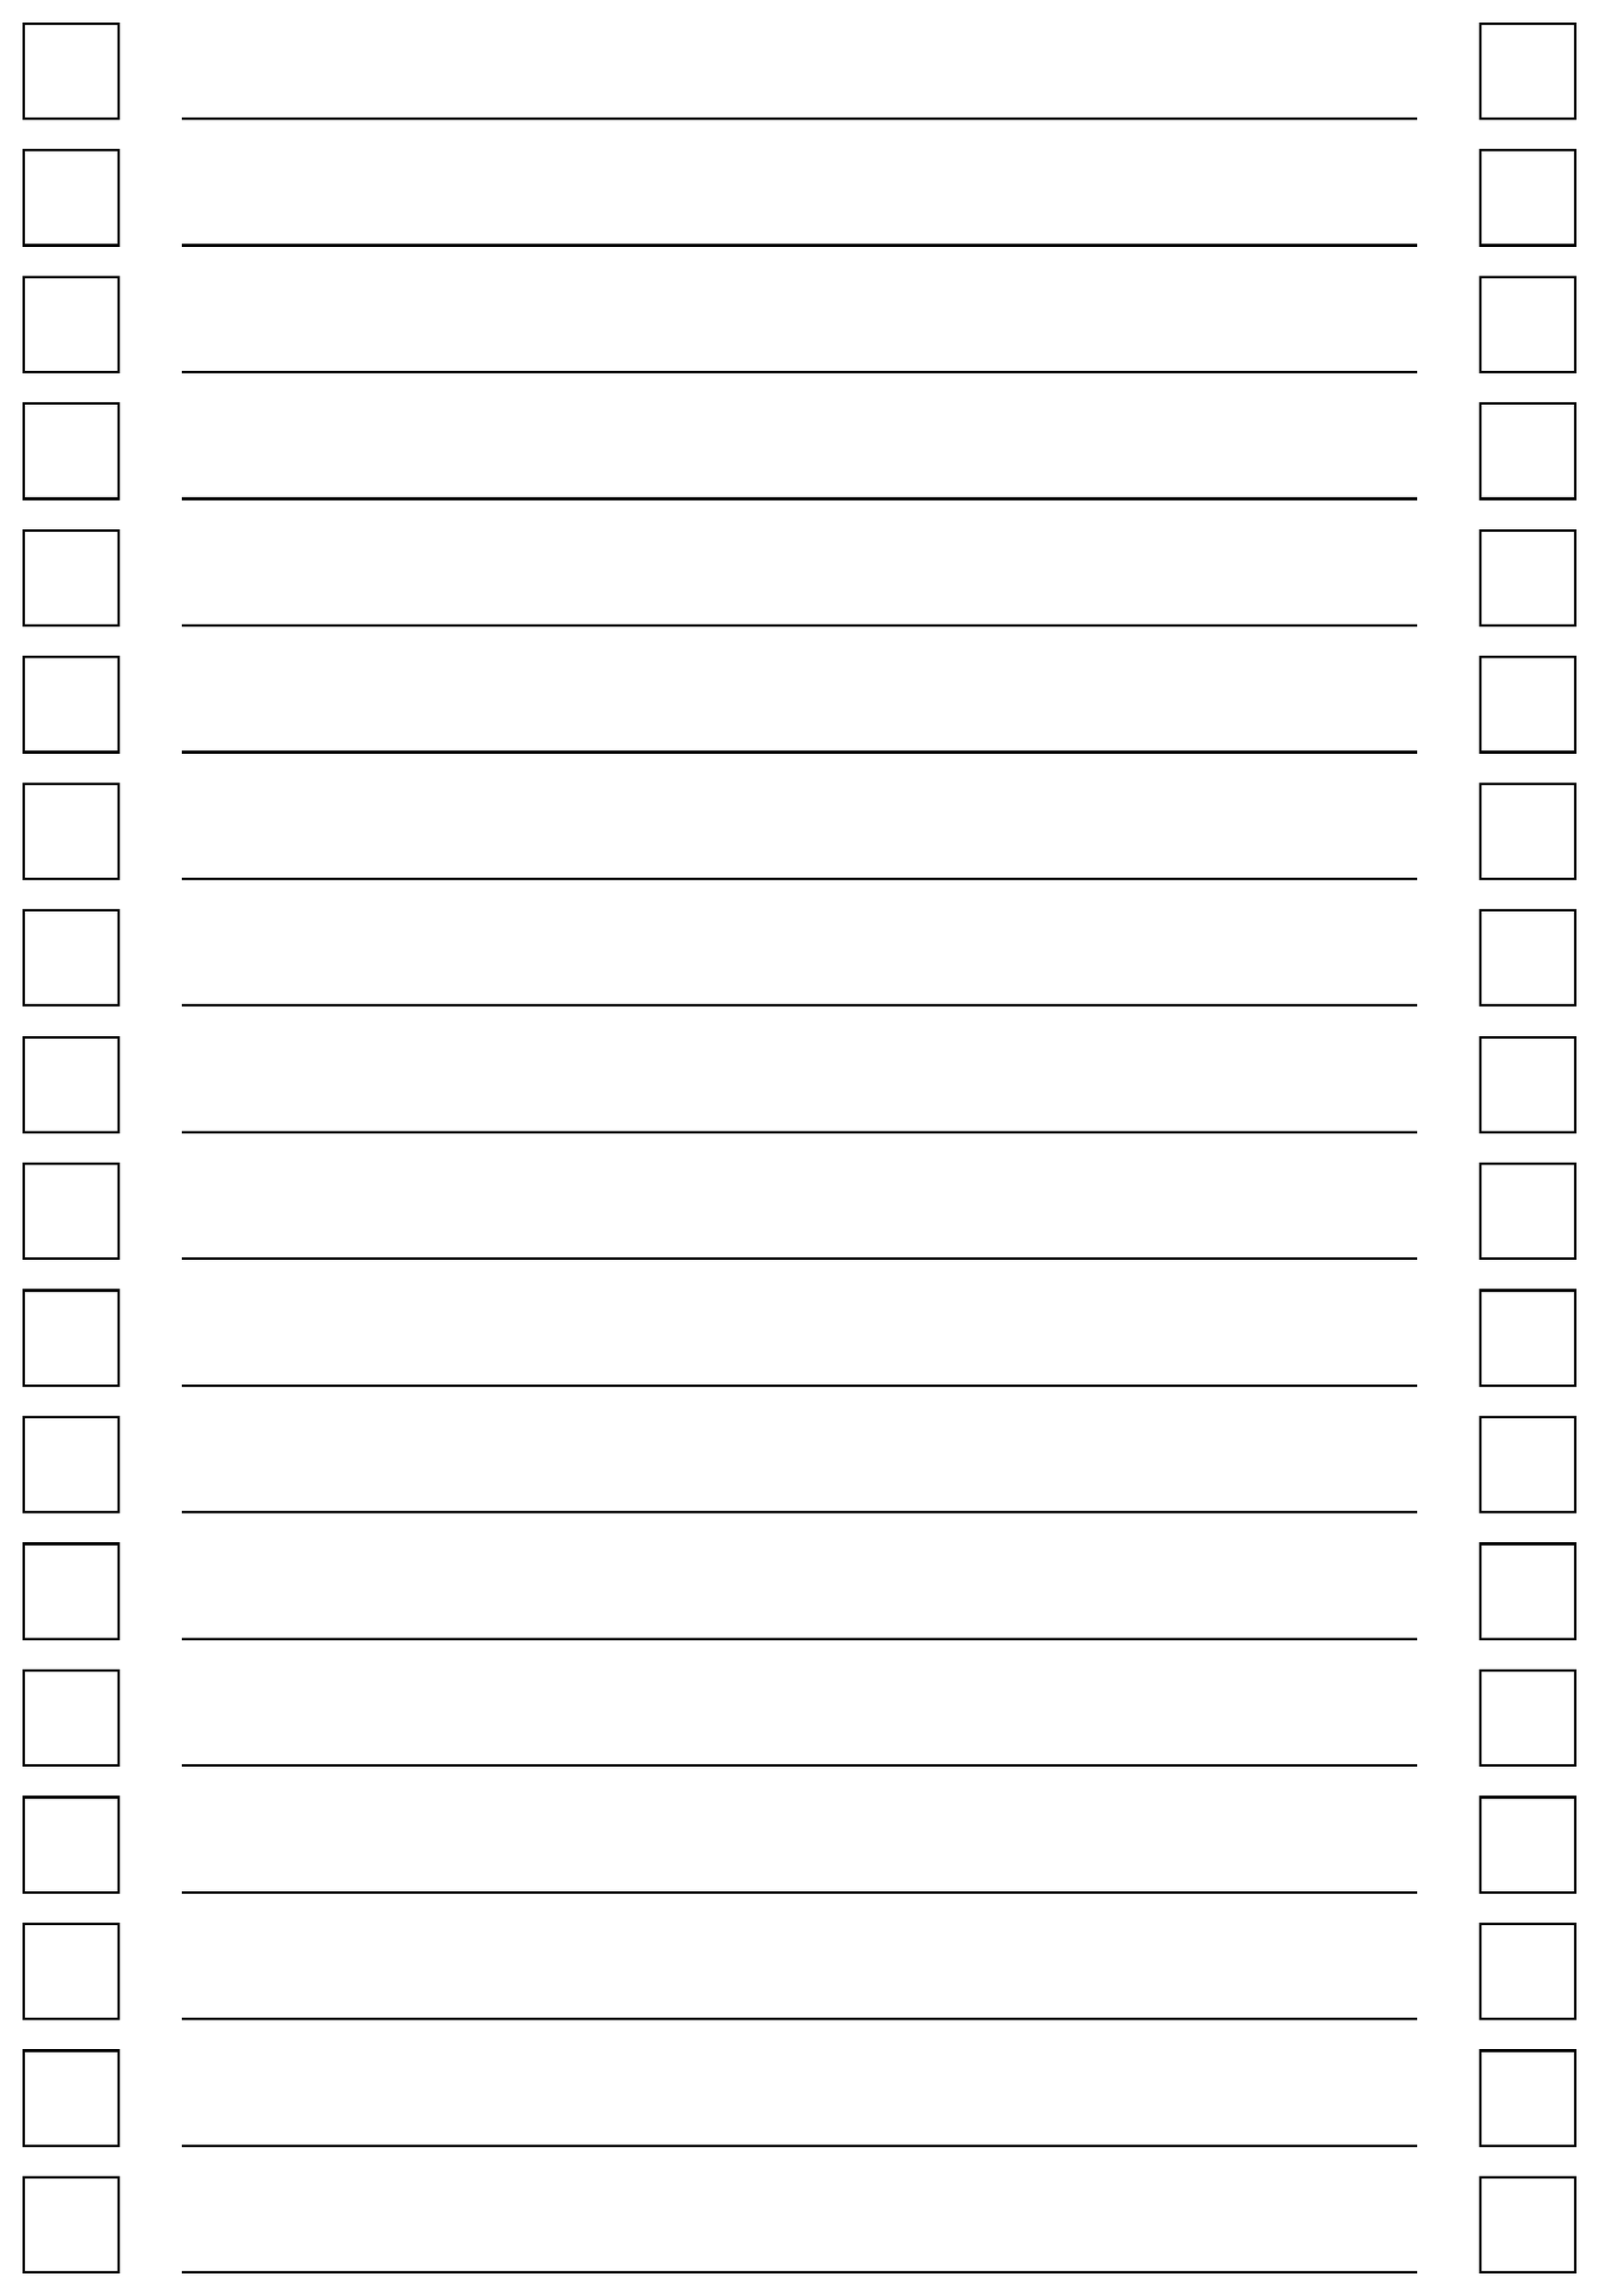
\begin{tikzpicture}
\foreach \i in {0,...,-17}{%
\draw[very thick](0,\i*2)-- ++(0,1.5)-- ++(1.5,0)
                            -- ++(0,-1.5)--cycle; 
\draw[very thick](2.5,\i*2)-- (22,\i*2);
\draw[very thick](23,\i*2)-- ++(0,1.5)-- ++(1.5,0) 
                             -- ++(0,-1.5)--cycle; 
}
\end{tikzpicture}
\clearpage
}
\end{lstlisting}

$\Rightarrow$ PDF mit 8-Seiten TODO-Liste

\end{frame}



\begin{frame}[containsverbatim]
\frametitle{Kombination mit \texttt{pgfpages} Code}

\begin{center}
\includegraphics[width=0.95\textwidth]{PocketMod_for_A3}
\end{center}

\end{frame}

\begin{frame}[containsverbatim]
\frametitle{Aktivitäts-Tracker I}

\begin{itemize}
	\item Aktivitäten wie \enquote{Katzenklo gesäubert?}, \enquote{2 Liter Wasser getrunken?}, etc
	\item pro Tag ein Pünktchen
\end{itemize}

\scalebox{1.1}{%
\lstinputlisting[morekeywords=,linerange={6-13}]{Tracker_Liste}}\vspace*{1em}

\end{frame}

\begin{frame}[containsverbatim]
\frametitle{Aktivitäts-Tracker II}

\begin{center}
\fbox{\includegraphics[height=0.8\textheight]{Tracker_Liste.pdf}}
\end{center}

\end{frame}


\begin{frame}[containsverbatim]
\frametitle{Kombination mit Python}

Idee: a) Monatskalender erzeugen und b) mit Events aus Google Calendar befüllen $\Rightarrow$ Python nutzen, um LaTeX zu erzeugen

Python: 
\begin{itemize}
\item eine Skriptsprache, erfunden in den Niederlanden
\item leicht erlernbar, kompakt, aber sehr mächtig
\item erlaubt objektorientierte, funktionale und Batch-Programmierung
\item Standard im Bereich ML und KI
\item Fokus auf lesbaren Code
\end{itemize}


\end{frame}

\begin{frame}[containsverbatim]
\frametitle{Monatskalender Teil 1}

Ziel: 2-dimensionales Array mit Wochen und Tagen, \\ Beispiel für den September 2021:

\begin{verbatim}
[['  ', '  ', '01', '02', '03', '04', '05'],
 ['06', '07', '08', '09', '10', '11', '12'],
 ['13', '14', '15', '16', '17', '18', '19'],
 ['20', '21', '22', '23', '24', '25', '26'],
 ['27', '28', '29', '30', '  ', '  ', '  ']]
\end{verbatim}
\end{frame}

\begin{frame}[containsverbatim]
\frametitle{Monatskalender Teil 1}

\scalebox{0.96}{%
\lstinputlisting[language=Python,linerange={6-26}]{cal-00.py}}

\end{frame}

\begin{frame}[containsverbatim]
\frametitle{Monatskalender Teil 2}

\scalebox{1.2}{%
\lstinputlisting[language=Python,morekeywords={join},linerange={28-34}]{cal-00.py}}\vspace*{1em}

%\begin{verbatim}
\begin{tabular}{ccccccc}
Mo & Di & Mi & Do & Fr & Sa & So \\
   &    & 01 & 02 & 03 & 04 & 05 \\
06 & 07 & 08 & 09 & 10 & 11 & 12 \\
13 & 14 & 15 & 16 & 17 & 18 & 19 \\
20 & 21 & 22 & 23 & 24 & 25 & 26 \\
27 & 28 & 29 & 30 &    &    &    \\
\end{tabular}
%\end{verbatim}


\end{frame}

\begin{frame}[containsverbatim]
\frametitle{Monatskalender Teil 3 - TikZ Version}

\begin{itemize}
	\item Schönere Kalender mit Tikz
	\item Einzelne nodes mit Position und Inhalt
	\item Formatierung über Stildefinition
\end{itemize}

%\scalebox{1.3}

\scalebox{0.96}{%
\lstinputlisting[language=Python,linerange={35-38}]{cal-00.py}}


\end{frame}

\begin{frame}[containsverbatim]
\frametitle{Monatskalender Teil 3 - TikZ Version}


\scalebox{0.96}{%
\lstinputlisting[language=Python,linerange={40-45}]{cal-00.py}}


\end{frame}

\begin{frame}[containsverbatim]
\frametitle{Monatskalender Teil 3 - TikZ Version Ergebnis}

\begin{center}
\fbox{\includegraphics[height=0.7\textheight]{tikz.png}}
\end{center}

\end{frame}

\begin{frame}
\frametitle{Google Calendar API}

API für Google Calendar

\begin{itemize}
\item Account unter \url{https://console.cloud.google.com}, Projekt erzeugen, Anmeldedaten erzeugen, OAuth 2.0-Client-ID erzeugen, Credentials.json herunterladen
\item \url{https://developers.google.com/calendar/api/quickstart/python}
\item 
\item 
\item 
\item 
\item 
\end{itemize}
\end{frame}

\end{document}